\documentclass[pageno]{jpaper}

\newcommand{\IWreport}{2017}
\newcommand{\quotes}[1]{``#1''}


\widowpenalty=9999

\usepackage[normalem]{ulem}
\usepackage[nottoc,numbib]{tocbibind}
\usepackage{minted}


\graphicspath{{images/}}
\usemintedstyle{emacs}

\begin{document}

\title{Encoder / Decoder Neural Networks for Protein Secondary Structure Prediction}

\author{Christopher Ferri\\Adviser: Professor Mona Singh}

\date{}
\maketitle
\thispagestyle{empty}
\begin{abstract}
In this thesis, I attempt to apply Encoder / Decoder neural networks to the problem of protein secondary structure prediction.  I explain the design of basic Recurrent Neural Networks and the history of secondary structure prediction algorithms.  I then describe the three network models that I will train and test, along with a simple test dataset built from the Protein Data Bank.  Through this study, I hope to provide a simple, accurate system for researchers to predict the secondary structure for a novel protein.
\end{abstract}

\begin{figure}
	\centering
	
\includegraphics[scale=0.75]{ShieldColor.pdf}
\end{figure}

\pagebreak
\doublespacing

\renewcommand{\abstractname}{Acknowledgements}
\begin{abstract}
Over the course of this year, many people have helped me along the way with the writing of this thesis.  Whether their contribution was large or small, I would like to take the time to thank them for their contributions.

\par
I would first like to thank my advisor, Professor Mona Singh, in the Lewis-Sigler Institute for Integrative Genomics for supporting my research.  I would also like to thank my second reader, Professor Sebastian Seung, of the Princeton Neuroscience Institute.

\par
I would like to thank my friends, who have been great resources.  My friend, Stephen Timmel, for helping me debug my preprocessing code.  My friends Matthew Penza and Stephen Bork, who have been great working buddies and proofreaders.

\par
I would like to thank my family.  My mother and Father, Roseann and John Ferri.  Thank you for all of the times you were willing to let me rant and rave about the latest step of producing a thesis, along with all the countless other ways you have supported me from a young age.  I wouldn't be here with out you guys.  My brother, Nicholas Ferri, for always knowing how to put a smile on my face and helping me to forget about my work, even for just a moment.

\par
I would like to thank the Roman Catholic church.  My years of being a practicing Catholic have taught me not only how to reason, but how to turn even my very work into a prayer.  You have giving me strength through the toughest of times, even when writing a thesis.

\par
\centerline{Ad majorem Dei gloriam inque hominum salutem.}
\centerline{J.M.J}
\end{abstract}

\pagebreak


{
\hypersetup{linkcolor=black}
\tableofcontents

\vspace{2pc}
\listoffigures
\listoflistings
}
\pagebreak



\section{Introduction}
Protein Secondary Structure prediction is one of the many open problems in Structural Biology.  Due to the inherent complexity of the problem, it is not solvable by any known closed-form equation; in fact, we will most likely never find any such solution.  Unfortunately, this information can be incredibly valuable to structural biologists, as the structure of the protein affects nearly all of its properties.  Due to the recent boom in Machine Learning methods, biologists have turned to Computer Science to help advance the current state of Secondary Structure prediction.  Many methods have pushed the accuracy into the 80\% range.  However, considering the complexity of chemical reactions that proteins participate in, this is not nearly accurate enough.  In this paper, state of the art techniques from Natural Language Processing and Deep Learning are put to use to help advance the state of the art in the field, and improve the accuracy of secondary structure prediction.  Using techniques such as word embeddings and Encoder / Decoder networks, we hope to increase the Q8 accuracy of prediction, resulting in a new method for protein secondary structure prediction.

\par
Currently, the process for discerning protein structure, secondary or higher, is a complex, expensive, and time consuming process.  In the age of high throughput sequencing, this is a bottleneck.  Research in the field of structural biology depends on understanding the complex form of a protein to perform research on the metabolic pathways that the respective protein is a part of.  By improving secondary structure prediction methods, we give biologists the ability to produce working drafts of the protein that they are studying, which can be used until experimental methods can be used to correct and verify the protein structure.

\section{Background}
In biology, all cells consist of a few classes of molecules: Lipids, Carbohydrates, Nucleic Acids, and Proteins.  Lipids and Carbohydrates are used for the structure of the cell, such as the cell wall, and energy.  Nucleic Acids make up our DNA and RNA, which encode Proteins and other regulatory information in the permutation of the nucleotides contained within them.  Proteins are the workhorses of the cell.  Their functions range from acting as catalysis for chemical reactions happening within cells, to forming complex channels in the cell membrane to allow specific molecules such as water to flow in and out of the cell.

\par
In what is considered the Central Dogma of Biology, genetic information is transcribed from DNA into mRNA.  From here, mRNA is translated from the sequence of chemical labels, called codons, into a long polymer, called a polypeptide.  Polypeptides are the building blocks of proteins; they go on to form proteins by organizing themselves into complex geometries that allow very specific proteins or chemicals interact with them.  Each of these polypeptides are composed of small, discrete chemical units called amino acids.  Like links in a chain, these amino acids chemically bond to form the long polypeptide.  In total, there are 20 canonical amino acids, each having unique properties that when combine in a specific order, determine the final geometry of the polypeptide, and in turn, the protein.  These 20 amino acids are displayed below in Figure \ref{fg:amino}, along with some of their properties, and their unique alphabetical letter which identifies each respective protein.  While there are 20 canonical amino acids, there exist a handful of non-canonical amino acids that do not correspond deterministically to a specific set of RNA codons.  Selenocysteine is one such of the non-canonical amino acids.  This translation is dependent upon the addition of a Selenocysteine Insertion Sequence (SECIS) in the mRNA \cite{longtin:2004}.  For the purposes of this study, we will ignore all but the canonical amino acids.  The unique structure of a protein is the result of countless electrostatic forces between the atoms within individual amino acids.  Through random changes in the protein shape, the take on their final configuration, which is an equilibrium between all of the atomic forces, to form a stable protein.

\begin{figure}[H]
	\centering
	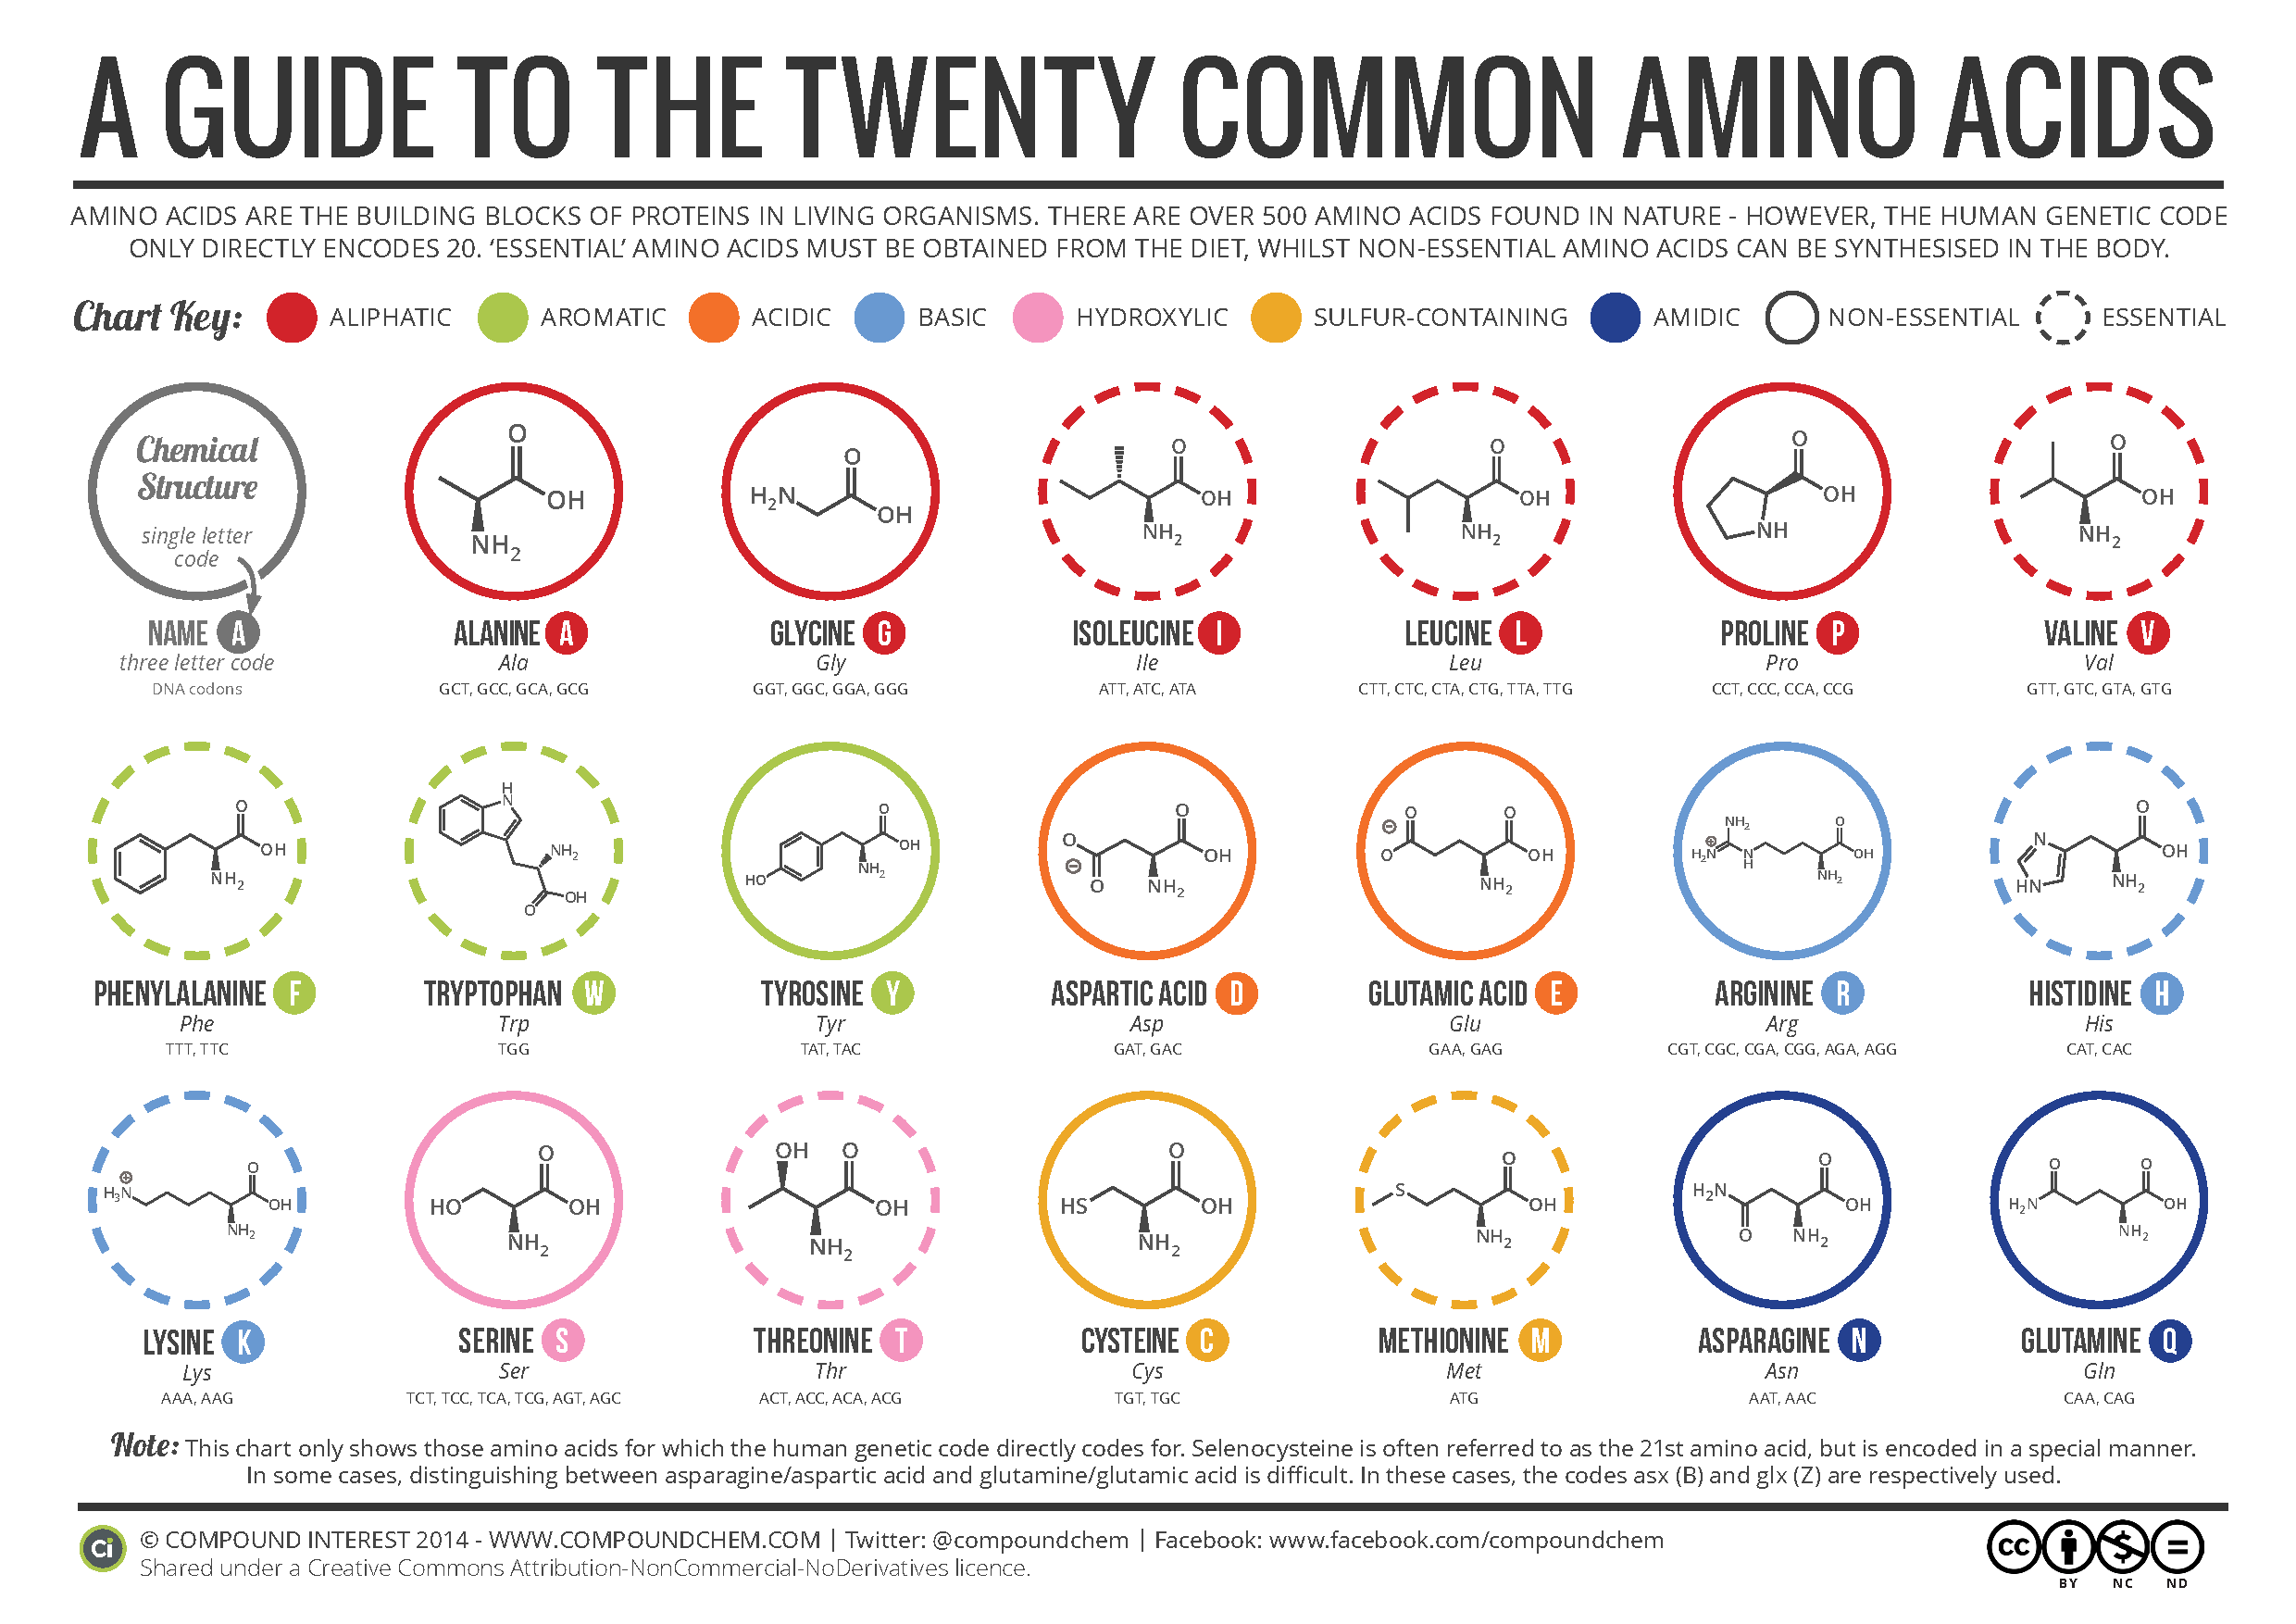
\includegraphics[trim={35pt 0 35pt 0}, scale=0.42]{20-Common-Amino-Acids-v2.pdf}
	\caption{The 20 canonical amino acids and their properties \cite{brunning:2014}}
	\label{fg:amino}
\end{figure}


\subsection{Protein Structure}
Protein structure can be divided into four levels: Primary, Secondary, Tertiary, and Quaternary.  Primary Structure is the sequence of amino acids that make up the polypeptide.  As previously stated, there are 20 canonical amino acids.  Secondary Structure is the formation of geometrical structures, such as $\alpha$-Helices and $\beta$-sheets, in the polypeptide.  Tertiary Structure is the large-scale configuration of the individual secondary structures and how they fit together to form a working protein.  Quaternary structure is the assembly of multiple polypeptides together to form a larger, more complex protein.  However, not all proteins are made up of multiple polypeptides; as such, not every protein has Quaternary Structure.  Figure \ref{fg:protstruc} below depicts the relationship between each of these levels of protein structure.


\begin{figure}[H]
	\centering
	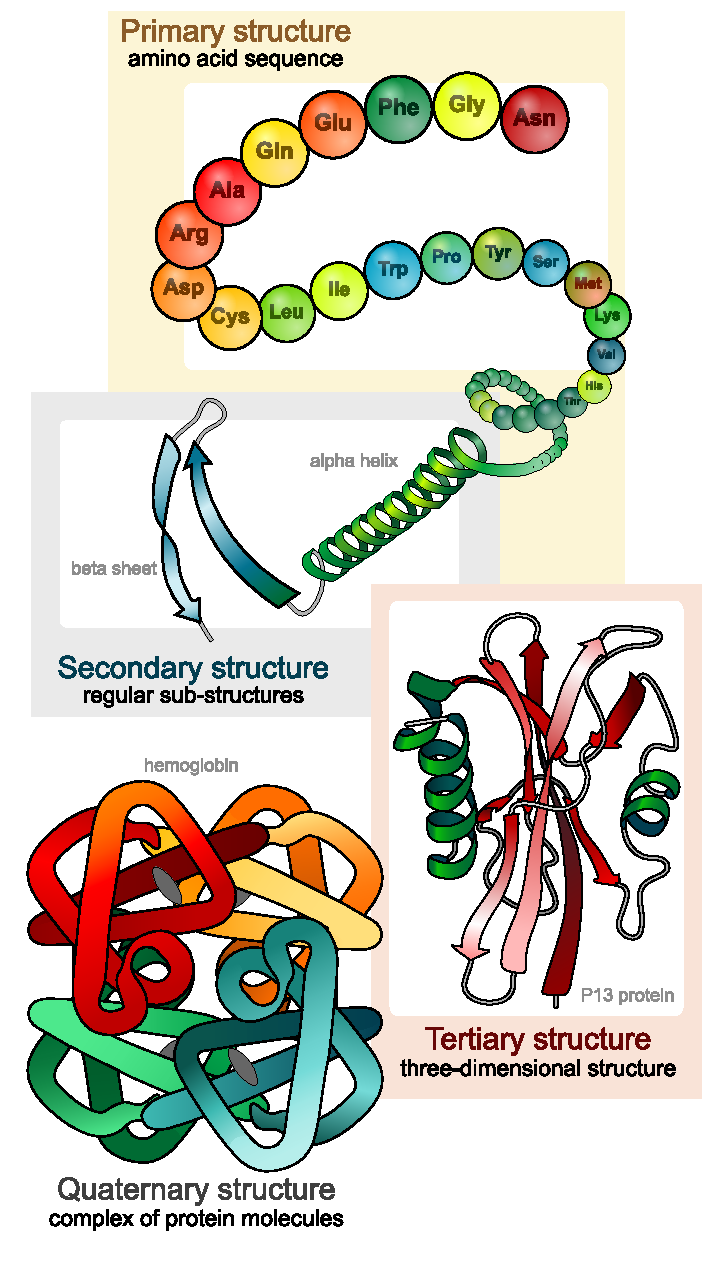
\includegraphics[scale=0.62]{ProteinStructure.pdf}
	\caption{A graphical breakdown of the four levels of protein structure \cite{wiki:2008}}
	\label{fg:protstruc}
\end{figure}

\par
To discover the structure at each respective level, scientists must use a combination of different methods to pool the data.  Primary structure is easily found through either protein sequencing techniques or by transcribing sequenced DNA which encodes the protein.  Much like DNA sequencing technology, it has become cheaper, faster, and more widely available.  Furthermore, the accuracy of current sequencing methods are well within the acceptable amount of error for scientific studies.  This leaves no need for any sort of predictive methods.  Conversely, Quaternary, Tertiary and Secondary structure are much more difficult.  The reason for this lies in the fact that both of these levels are related directly to the geometric layout of the polypeptide vs. the chemical composition.  To find the geometrical structure of a protein, scientists must crystallize the protein and use techniques such as X-Ray Crystallography, Nuclear Magnetic Resonance Spectroscopy (NMR), or Cryo-electron microscopy to find the positions of atoms with respect to each other.  For example, in the case of X-Ray Crystallography, large amounts of X-Ray radiation from a Synchrotron are shined through a crystallized protein.  By recording the diffraction pattern, scientists are able to reassemble the 3 dimensional structure of the protein.  From there, they are able to hand annotate the protein to create a finalized model of the protein.  However, there are a couple of downsides to this process, specifically the process of crystallizing a protein and the requirement of a Synchrotron.  Crystallizing a protein is a process that can take months at a time, and requires the protein to form without any imperfections, otherwise there won't be a diffraction pattern.  Moreover, Synchrotron sources are very large and expensive, requiring researchers to travel to a national laboratory to run the experiments.  NMR does not crystallization of the protein, and the equipment to run the experiment can be found in many large research universities.  By using the same technology as MRI scanners, NMR machines use large magnetic fields to direct the molecule in two directions parallel to the magnetic field.  From there, large radio waves bombard the molecules, causing them to selectively flip direction.  By recording the frequency when these flips occur, we can identify the structure of the molecule.

\subsection{Neural Networks}
Neural networks are a machine learning technique that originated with the invention of the Perception by Frank Rosenblatt \cite{rosenblatt:1958}.  The Perceptron is a device for binary classification.  Its input consists of a single vector $\vec{x}$ and a binary output $y$.  Inside, it contained a weight vector $\vec{w}$ which was learned during the training phase.  Mathematically, it can be represented by Equation \ref{eq:neuron}:
\begin{equation}
	\label{eq:neuron}
	y = f\left(\sum_{i = 0}^{n} w_{i}x_{i} + b\right)
\end{equation}

The function $f(u)$ is usually either the Heaviside step function, the Sigmoid / Logistic function, $\tanh$ function, or RelU.  Each of these functions operate such that their range is $\{u \in \mathbb{R} : -1 \leq f(u) \leq 1\}$, with the exception of ReLU, which has a range of $\{u \in \mathbb{R} : 0 \leq f(u)\}$.  This allows for easy binary classification.  However, it has been shown that Perceptrons, including multi-neuron versions, have very strong limitations.  For example, while a Perceptron can learn most boolean functions, it has been proven that there is no way for a Perceptron to internally represent the XOR function with any set of values for $\vec{w}$ and $b$.  Neural networks take this idea of a Perceptron and generalize them with more of them and by stacking them together.  To train them, we use an optimization technique known as Stochastic Gradient Descent.  To allow the Gradient Descent to update all layers of the network, an algorithm known as backpropagation, which is based off of the derivative chain rule, allows weight updates to be propagated backwards through the network.  The algorithm first calculates $\delta_{i}^{L}$, where subscripts represent individual neurons, and the superscript $L$ represents the last layer.  This value is the gradient of the output layer, for any general error function $e$.  This is calculated via the equation $\delta_{i}^{L} = f'\left(u_{i}^{L}\right) \frac{\partial e}{\partial x_{i}^{L}}$, where $u$ is the preactivation of the neuron, the result of the dot product between the $\vec{w}$ and $\vec{x}$ vectors.  Given this first gradient, we are able to iteratively calculate the weight updates for each layer by using Equation \ref{eq:backprop} \cite{seung:2017}:
\begin{subequations}
	\label{eq:backprop}
	\allowdisplaybreaks
	\begin{gather}
	\delta_{j}^{l - 1} = \left(\sum_{i = 1}^{n_{l}} \delta_{i}^{l} W_{ij}^{l} \right)  f'\left(\vec{u}^{l}\right) \\
	\Delta\mathbf{W}_{ij}^{l} = \eta \delta_{j}^{l} x_{i}^{l - 1} \\
	\Delta b_{i}^{l} = \eta \delta_{j}^{l}
	\end{gather}
\end{subequations}

\par
One of the main difficulties with neural networks is processing long sequences of data.  As it is unable to take the entire input in at once, the network must process small blocks of the sequence at a time.  This leads to a problem; the network is unable to take previous information / context into account when making inferences on the data.  Recurrent Neural Networks (RNN) were created to solve this problem.  An RNN is designed to process long sequences of data, such that the network can take into account information from a previous part of the sequence, at the current moment.  The key to this ability is that each RNN neuron produces not only an output, but a hidden state that is then passed back into the cell.  This information contains the necessary information for the cell to take context into account during classification.  Below, Figure \ref{fg:rnn} is a diagram that shows this feedback loop, and how it is equivalent to information being passed down to cells that process inputs of the sequence later on.

\begin{figure}[H]
	\centering
	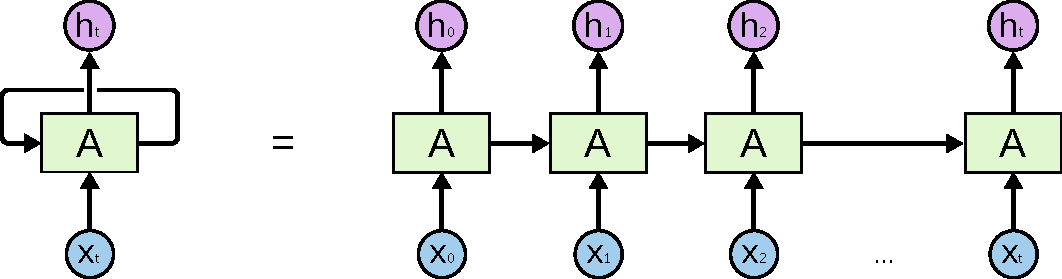
\includegraphics[scale=0.9]{unrolledRNN.pdf}
	\caption{An Unrolled RNN \cite{olah:2015}}
	\label{fg:rnn}
\end{figure}

To train the network, we must use a modification of backpropagation, called backpropagation through time.  This algorithm propagates errors not only backwards through the network, but backwards through the feedback loop, so as to allow the network to update through the feedback loops.  In terms of taking the gradient, the feedback loop is treated as a deeply nested function, requiring only the chain rule to provide the correct gradient.  To improve training time and improve accuracy, backpropagation through the feedback loop is truncated to a finite number of passes.

\par
However, there is an inherent problem with this model of an RNN.  Called the Vanishing Gradient Problem, as the backpropagation through time algorithm proceeds through though the feedback loop, the activation function causes the gradient to exponentially decay \cite{bengio:1994}.  This causes the network to have problems recognizing long term relationships in sequences.  In modern RNN's, the problem is solved by using cells that are very different from that of a standard feedforward neural network.  The most common type of cell is called a Long Short Term Memory cell \cite{hochreiter:1997}.  Each cell contains multiple logic gates, called forget gates, which allow it to control the flow of previous information in future time steps of the network.  They also prevent the exponential decay of the gradient, allowing the network to be properly trained.

\begin{figure}[H]
	\centering
	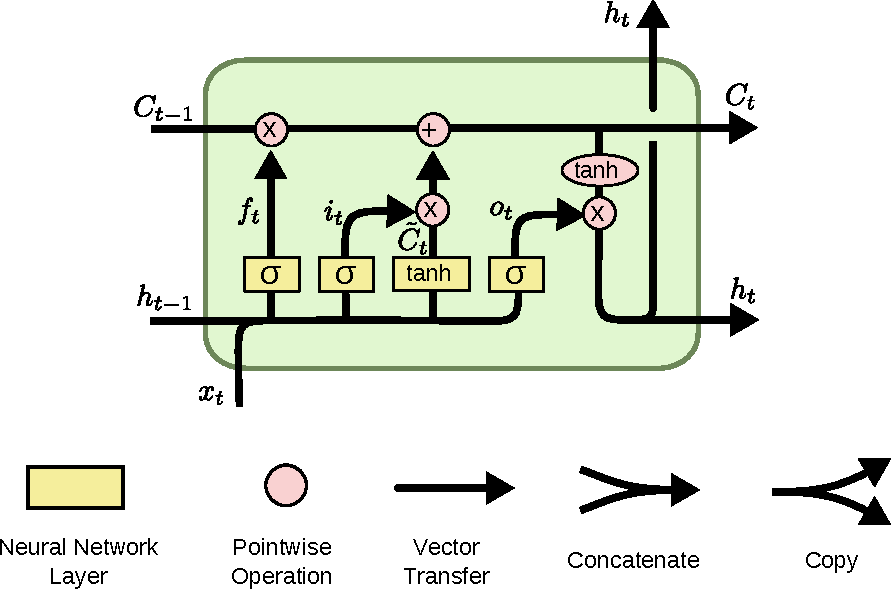
\includegraphics[scale=0.75]{LSTM.pdf}
	\caption{An LSTM Cell \cite{olah:2015}}
	\label{fg:lstm}
\end{figure}

As depicted above in Figure \ref{fg:lstm}, an LSTM cell has two hidden states that each uniquely transmit information through pointwise operations with the input and the previous hidden states.  Most RNN's today use some version the LSTM architecture, but as of 2014 a simpler architecture called a Gated Recurrent Unit (GRU) has been gaining popularity in the research community \cite{cho:2014}.

\subsection{Secondary Structure Prediction}
Secondary structure prediction is the process of predicting the conformation of a polypeptide string given any valid polypeptide string.  This conformation takes the form of either a $\alpha$-helix or $\beta$-sheet.  For secondary structure, each amino acid can take on only 1 conformation, out of a specified set of conformations.  This makes secondary structure prediction an inherently more tractable problem than tertiary structure prediction.  While tertiary structure prediction requires an algorithm to predict the 3 dimensional location of each atom of the polypeptide, secondary structure prediction is only required to apply a label of conformation to each amino acid.  This is a well known problem in machine learning, known as classification.

\par
One of the earliest methods for secondary structure prediction was the Chou-Fasman method, proposed in 1974 \cite{singh:2005}.  This method simply calculated the probability of every amino acid being part of an $\alpha$-Helix, a $\beta$-Sheet, or neither, normalized for the number of times the respective amino acid appears.  This method, while a good beginning step, was very simplistic and naive.  First and foremost, it does not take the surrounding amino acids into account for a particular protein, making it impossible to use previously predicted structure states to make the current prediction.  Furthermore, it does not account for long range interactions that help to stabilize the $\alpha$-helix and $\beta$-sheet structures.

\par
Later, in 1978, the GOR method improved the approach and created a mathematical formalization of the problem \cite{singh:2005}.  The key was to define the problem in terms of information theory; each amino acid is viewed in context of the whole amino acid sequence, with the goal for each amino acid being to predict the conformation type with the highest information \cite{garnier:1978}.  Mathematically, this goal appears as $\underset{S_{i}}{\arg\,\max} \ I(S_{i}:R_{i - j}, R_{i - j + 1}, R_{i - j - 2} \ldots R_{i + j - 2}, R_{i + j - 1}, R_{i + j})$, defining information as the following in Equation \ref{eq:gor}:
\begin{equation}
	\label{eq:gor}
	I(y:x) = \log\left(\frac{\Pr\left(y \vert x\right)}{\Pr(x)}\right)
\end{equation}

To fully calculate this value would be impossible even on todays computers.  To over come this, a simple approximation is put forward in Equation \ref{eq:resapprox}:
\begin{equation}
	\label{eq:resapprox}
	I(S_{i}:R_{i - j}, R_{i - j + 1}, R_{i - j - 2} \ldots R_{i + j - 2}, R_{i + j - 1}, R_{i + j}) \approx \sum_{j = -n}^{n} I(S_{i} : R_{i + j})
\end{equation}

This simplification allows us to calculate the information given by each amino acid surrounding the current amino acid.  To further simplified the problem, instead of taking all other amino acids into account, one can specify a small window of size $m$ such that $m < n$, dropping the total number of information residues to be at max $2m$.  In the original paper, they choose $m = 8$ as their window size, which means the surrounding 13 amino acids inform the prediction of the current amino acid configuration.  While this method addresses the problem of taking surrounding information into context, it fails to examine the configuration of the surrounding amino acids.

\par
Other approaches that have been tried include nearest neighbor algorithms, which attempt to use nearest neighbor based classifiers by taking the current amino acid with the surrounding amino acid, and using the algorithm to identify other amino acid sequences that are similar and have been labeled with their conformation.  By examining these sequences, the algorithm is able to give a predicted conformation for the amino acid.  This algorithm and extensions of the previously mentioned algorithms have achieved higher than 60\% accuracy, which is a significant improvement over the accuracy achieved with random guessing, but not enough to become a viable alternative to experimental structural prediction methods \cite{singh:2005}.

\par
Starting in 1989, neural network based methods started to come into practice.  These networks were very shallow and simple in contrast to today's ever deepening networks.  One of the most successful neural network approaches was that of Rost and Sander \cite{rost:1993}.  This method used a 2 layer neural network that included a multiple alignment of the protein against other similar proteins.  The first layer would examine different sections surrounding the current amino acid being classified, and proceeds to classify the structural conformation of these independent, surrounding sections.  The second layer takes these independent predicted conformations and then processes them to predict the conformation of the current amino acid.  Finally, a jury decision layer to help reduce noise in the neural network architecture, after which the highest conformation class is used as the predicted conformation.  This method was able to achieve an accuracy of 70.8\% accuracy for basic 3-state secondary structure prediction.

\par
Currently, neural networks are replacing previous generation methods such as Hidden Markov Models.  One of the most recent attempts is that of Wang, Peng, and Xu \cite{wang:2016}.  This proposed an algorithm called DeepCNF (Conditional Neural Field); this algorithm was derived from standard neural networks and a Conditional Random Field (CRF), an algorithm associated with prediction and classification on a sequence.  A traditional CRF allows for prediction, while taking previous and forward context into account.  Using this information, it uses a simple linear classifier to make its prediction.  In the case of DeepCNF, the linear classifier is replaced with a convolutional neural network.  In their paper, Wang et al. test multiple network architectures, of 1, 3, 5, and 7 layers, with the 7 layer model giving the best 8-state accuracy.  In summary, they were able to achieve a 3-state accuracy of 84.7\% and an 8-state accuracy of 72.3\%.

\par
Despite this constantly improving accuracy, there are limits to using algorithmic based methods to predict secondary structure in proteins.  In fact, it is estimated that there exists an upper limit of accuracy around 88\% \cite{rost:2001}.


\section{Approach}

\subsection{Encoder / Decoder Architecture}
While Recurrent Neural Networks as described above are great for processing sequences, they are only able to output a single value for the entire sequence.  For example, in the case of sentiment analysis, a Recurrent Neural Network is able to process a sentence then provide a single number to rate the sentiment inherent to the sentence as either good or bad and how good or bad it is.  This is useful for many problems.  However, in the field of machine translation, more than one output is required.  In fact, an entire sequence is the output.  This lead to the creation of Encoder / Decoder, known more colloquially as Seq2Seq models, which allows translation from one sequence to another \cite{cho:2014}.  It consists of two Recurrent Neural Networks placed together, with one focused on learning the input sequence representation, called the Encoder, and the second RNN, called the Decoder, is focused on outputting a translation of the sequence.  This technique has been shown to be highly successful at Machine Translation, and is being used as the new translation algorithm for Google Translate \cite{wu:2016}.  This network is shown depicted below in Figure \ref{fg:enc_dec}.
\begin{figure}[H]
	\centering
	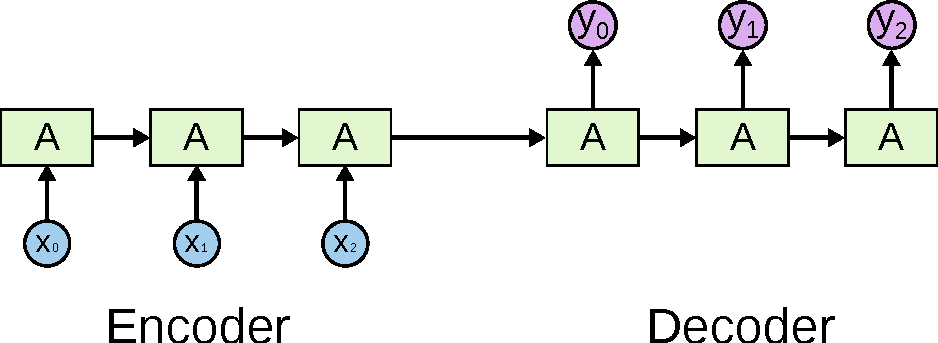
\includegraphics[scale=1.0]{encoder_decoder.pdf}
	\vspace{1pc}
	\caption{An Encoder / Decoder RNN a single layer for each \cite{olah:2015}}
	\label{fg:enc_dec}
\end{figure}

As we can see, Figure \ref{fg:enc_dec} depicts the Encoder processing the input data $X_{1}, X_{2}, X_{3}$ and learns the inherent meaning of the input.  From there, the Encoder feeds that information as a vector into the Decoder, where the Decoder is able to take the meaning of the sequence and translate it into the language that it has been trained for.  As it is a Recurrent Neural Network, it is trained by the Backpropagation through Time algorithm (BTT), but usually takes longer than a standard RNN, due to the fact that two networks that must be trained.  For the problem of translation, we have the Equation \ref{eq:ed_loss} as the loss function for the network.

\begin{equation} \label{eq:ed_loss}
	\underset{\theta}{\max} \frac{1}{N} \sum_{i = 1}^{N} \log(P_{\theta}(y_{i} \vert x_{i}))
\end{equation}

With this loss function, we can see that for the model parameters $\theta$, we are trying to optimized the log loss probability that $y_{i}$ will appear given $x_{i}$ for all $i$.  Overall, this means that the neural network will learn to mimic the translated output, given the input.

\par
For this study, we will be using a modification of the basic Encoder / Decoder algorithm.  One of the problems with a standard Recurrent Neural Network is the fact that it can take past context into account, but not future context.  Future information can be just as important as past information, especially in the case of secondary structure, where all of the surrounding amino acids affect the structure of a given amino acid.  To allow for RNNs to account for this future context, Bidirectional RNNs were created.  First proposed in 1997, the network incorporates future context by doubling the number of hidden states in each RNN / LSTM cell, with half being for past conxtext and the other half being for future context \cite{schuster:1997}.  This means that an individual RNN / LSTM cell recives a forward and a backward hidden state, increasing the accuracy of the prediction.  This technique has been used successfully in protein secondary structure prediction algorithms, and have been found to do better than state of the art methods in 2005 \cite{pollastri:2005}.  This type of network is used within the Encoder of the Encoder / Decoder model.

\par
Given this recent architecture, I believe it will prove successful at predicting the secondary structure of proteins and rank very high in terms of accuracy of prediction.


\subsection{ProtVec}
An inherent problem processing vocabulary sequences is information sparsity.  Any given sequence may only contain a very small subset of possible words, each of which posses a complex relationship with many other words.  To counter this, a technique known as word embedding tries to compress this relational information into a continuous vector space \cite{mikolov:2013}.  In a word embedding system, each word is represented by a high dimensional vector, where the vector represents its relationship to other words in the high dimensional vector space.  One of the unique properties of a good embedding is the fact that relationships between words can be represented through vector arithmetic.  For example, in a good embedding the equation $\vec{w}_{Berlin} - \vec{w}_{Germany} + \vec{w}_{France} \approx \vec{w}_{Paris}$ holds, showing that within a word embedding, there exists a linear relationships between each word.  For this project, we hope to capture the relationships between three-mers in the protein sequences.

\par
While word embedding techniques have traditionally been used exclusively for natural language processing and machine translation tasks, they have been successfully applied to biological sequences.  Called BioVec, DNA and protein sequences can be successfully embedded in a vector space using the Skip-Gram model using three-mers as the words that make up the vocabulary of proteins \cite{asgari:2015}.  In this paper, researchers were able to represent the protein sequence using the three-mer embeddings as input features to an Support Vector Machine classifier, for the problem of protein family classification.  Researchers were able to achieve 93\% accuracy on this task.  This demonstrates that proteins sequences, like sentences, contain relational information between their three-mers / words.

\par
To build this embedding, we build a linear (without an activation function) neural network with a single hidden layer.  The input layer contains a number of neurons equal to the size of the vocabulary.  The hidden layer is represented by the embedding matrix.  Given this network, we use one of two possible algorithms, Continuous Bag of Words and Skip-Gram, to train the network and build the embedding matrix.  For this project, we will be using the Skip-Gram algorithm, as it produces better results with words in the vocabulary that are rare.  The algorithm can be described as training the neural network to predict the surrounding words, given an input word.  In the first variation of this algorithm, the log loss of the softmax equation was used as the error function, $J$ in Equation \ref{eq:softembed}

\begin{subequations}
\label{eq:softembed}
\begin{gather}
P(w_{c} \vert w_{t}) = \frac{e^{\vec{w_{c}} \cdot \vec{w_{t}}}}{\sum_{v \in Words} e^{\vec{v} \cdot \vec{w_{t}}}}\\
\log(P(w_{c} \vert w_{t})) = \left(\vec{w_{c}} \cdot \vec{w_{t}}\right) - \log\left( \sum_{v \in Words} e^{\vec{v} \cdot \vec{w_{t}}} \right) \\
J(W) = \frac{1}{T} \sum_{t = 1}^{T} \sum_{-c < j < c, j \neq 0} \log(p(w_{t + j} \vert w_{t}))
\end{gather}
\end{subequations}

However, this error function becomes intractable for large vocabularies, requiring on the order of $10^{5}$ to $10^{7}$ terms to be computed for each gradient \cite{mikolov:2013:2}.  To combat this, two methods, Negative Sampling and Noise Contrastive Estimation, were put forward as simpler error functions that achieve good embedding results \cite{mnih:2013}.  Although Negative Sampling might be considered to be the better methods, we will be using Noise Contrastive Estimation, due to its native implementation in TensorFlow.  Noise Contrastive Estimation reduces the number of parameters to learn by requiring that individual words be tested against the input word.  This can be represented by Equation \ref{eq:nce_loss} below, where the probability distribution produces the probability of a given word pair occurring together.  The equation uses the notation provided to us in the original paper by Minh and Kavukcuoglu.
\begin{subequations}
	\label{eq:nce_loss}
	\begin{gather}
	\sigma(x) = \frac{1}{1 + e^{-x}} \\
	\Delta s_{\theta}(w, h) = s_{\theta}(w, h) - \log(k P_{n}(w))\\
	P^{h}(D = 1 \vert w, \theta) = \sigma\left(\Delta s_{\theta}(w,h)\right)\\
	J^{h}(\theta) = E_{P^{h}_{d}}\left[\log \left(\sigma\left(\Delta s_{\theta}(w,h)\right)\right)\right] - kE_{P_{n}}\left[\log \left(1 - \sigma\left(\Delta s_{\theta}(w,h)\right)\right)\right]
	\end{gather}
\end{subequations}

This new error function approximates the logarithmic softmax output.  The only impediment to this is the requirement of the noise probability distribution, $P_{n}$.  This must be manually calculated by 

\section{Implementation}

\subsection{Models}
For this study, we test three models, a small model, a medium model, and a large model.  The first three models are pure Encoder / Decoder models and are the core of this study.  Each of these models are based off of the example models provided in the tf-seq2seq source code. For all models, we will use an embedding size of 128 for all models, as we do not need as large of a word embedding as networks used for language translation.  Moreover, we are using LSTM based cells in all of the Decoder networks and the first three Encoder networks.  All model configuration files can be found in the Appendix section of this paper.  The files contain a few other parameters that are not mentioned in this paper, but are taken from the configuration files that were included in the tf-seq2seq package.

\par
The small model was built with the primary motivation being to show basic evidence for the success of an LSTM based Encoder / Decoder system on the problem.  It consists of one Encoder layer and one Decoder layer.  This model will be very easy to train, and will only take a few hours.

\par
The medium model attempts to deepen the Decoder network to increase accuracy.  I consists of one Encoder layer and two Decoder layers.  This model will take a bit longer to train, and will probably take a whole day to train on the compute cluster. 

\par
The large model increases both the Encoder and Decoder depth.  It consists of two layers in the Encoder and four layers in the Decoder.  I expect to get the highest accuracy on this model, as it is the most complex.  However, this accuracy comes at the cost of a long training time. This model will take between one to three days to train for 5,000,000 steps.

\par
Moreover, there are multiple ways to test the accuracy of a secondary structure prediction algorithm.  The two most popular are Q3 and Q8 accuracy.  Simply put, these two accuracy measures simply tally the percent amino acids the algorithm correctly predicted.  Now Q3 and Q8 each use different labeling classes, with Q3 using the standard three secondary structure classes, $\alpha$-helix, $\beta$-sheet, and coil.  Q8 on the other hand, uses eight individual classes, which are subclasses of the Q3 structure types.  The Q8 classes are described in the Table \ref{tb:q8} below.

\begin{table}[H]
	\centering
	\caption{Q8 Classes as defined by PDB \cite{berman:2000}}
	\label{tb:q8}
	\begin{tabular}{|l|l|}
		\hline
		\textbf{Structure Letter} & \textbf{Structure Type}                               \\ \hline
		H                & $\alpha$-Helix                               \\ \hline
		B                & Residue in isolated $\beta$-bridge           \\ \hline
		E                & Extended Strand, participates in $\beta$-ladder \\ \hline
		G                & 3-Helix ($\frac{3}{10}$ Helix)               \\ \hline
		I                & 5-Helix ($\pi$ Helix)                        \\ \hline
		T                & Hydrogen Bonded Turn                         \\ \hline
		S                & Bend                                         \\ \hline
		C                & Coil                                         \\ \hline
	\end{tabular}
\end{table}

\subsection{Attention Mechanism}
A common mechanism that is used to enhance the predictive power of Encoder / Decoder architectures is the use of a technique called Attention.  First introduced by Dzmitry Bahdanau in 2014, this allows Encoder / Decoder networks to focus individual outputs from the Decoder on the pertinent inputs to the encoder \cite{bahdanau:2014}.  When translating a sentence, the translator focuses mostly on the current word and slightly on a few surrounding words, attention mechanisms attempt to mimic this by deemphasizing the output of Encoder cells that are farther away from the current word being translated.  This is accomplished by passing a vector, called the query vector, from the Decoder to the encoder.  Then we take the dot product of the query vector and the output vectors from the Encoder network, and put it through a softmax layer.  The output of the softmax is called the attention distribution, and decides which parts of the input are the most pertinent to the current decoder state.  From here, each scalar value is multiplied by their respective Encoder vector and summed together to get the final input to the the Decoder cell.  This process is depicted below, in Figure \ref{fg:attn}.  Note how for the Decoder cell certain Encoder vectors are weighted much more strongly.
\begin{figure}[H]
	\centering
	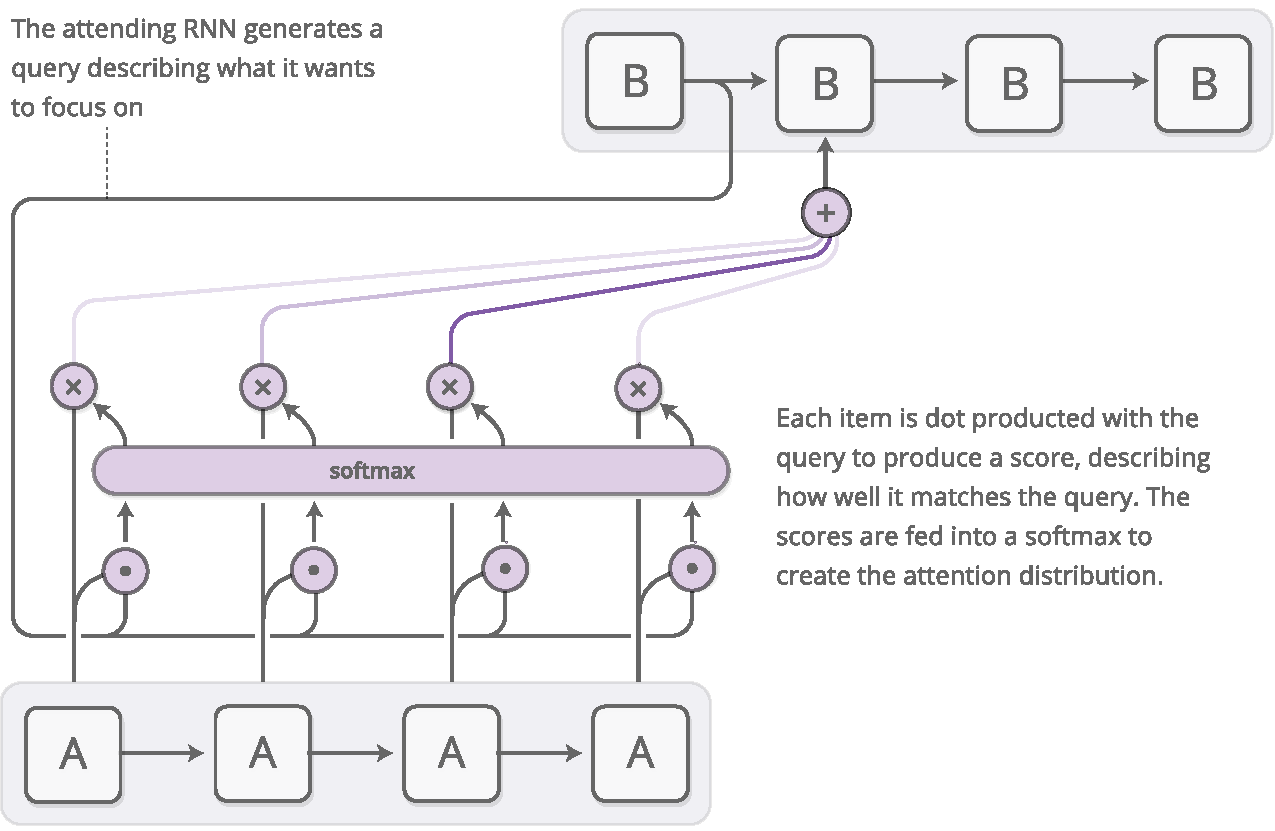
\includegraphics[scale=0.73]{attentionRNN.pdf}
	\caption{Attention Mechanism in an Encoder / Decoder network \cite{olah:2016}}
	\label{fg:attn}
\end{figure}

The addition of the attention mechanism has the benefit of allowing each Encoder state to output a vector of information for the Decoder instead of a single vector from the final output of the Encoder.  This increases the amount of information that is given to the decoder, allowing it to make better predictions.  In the three models we will be testing, the attention vector will be of length 128.

\subsection{TensorFlow}
One of the keys to implementing this project has been the Tensorflow library \cite{tensorflow:2015}.  Released by Google in 2015, the library focuses on providing an all inclusive neural network library.  The user is given many primitive operations to construct the network; this network must be defined before beginning the training phase, so that the library is able to pre-calculate the derivatives and compile the math expressions required for backpropagation through the network.  By doing this, the library is able to optimize the computation of both forward and backwards passes through the network.  As with every other major neural network library, it includes CUDA support, allowing GPU acceleration to greatly reduce training time.  One of the more unique features of the library is its new XLA accelerator.  XLA is a Just-in-Time (JIT) compiler, designed specifically for compiling high level graph operations together, so as to speed up both the training and inference times of the network.  Furthermore, all training data can be recorded, and easily accessed through the Tensorboard interface.  From here, we are easily able to export all scalar data (learning rates, gradient magnitude, and network cell parameters) via a CSV.  Instead of installing the vanilla TensorFlow package available from the Python package manager, I chose to compile TensorFlow from source, gaining me extra vector extensions and the XLA accelerator; these features will help to reduce training and inference time.  For this project, we will be using version r1.0, released on February 15, 2017.

\par
Running on top of Tensorflow is the newly released tf-Seq2Seq package \cite{britz:2017}.  Open-sourced on April 11, 2017, this package allows the user to build Encoder / Decoder networks with little, to no code.  The network architecture is passed into the program via a single YAML file that contains specifications such as the number of hidden layers, the type RNN cells to be used, learning rate, etc.  This helps to make model easy to distribute, as only a small set of files need to be provided to run a trained model.  One of the main benefits to using this package is that it natively supports multi-GPU acceleration, along with distributed computing among multiple compute nodes.  This allows the use of large clusters for training the model quickly.  Furthermore, this package helps to improve reproducibility, by standardizing the code and providing the precise hyper-parameters in a small number of configuration files.  The data is fed into the network via two separate files, the source and target files, which are in Parallel Text Format.  With the release of this package, all but my preprocessing code was made obsolete.  As such, I quickly re-factored my entire software pipeline to incorporate this package.

\subsection{Regularization}
One of the problems we come across when training a neural network is the problem of overfitting.  This occurs when the network begins to learn specific examples in the training dataset instead of learning the ground truth behind the data it is classifying.  This is easily detected through the use of a validation dataset.  If the training error and the validation error diverge, with the validation error beginning to plateau or increase, then overfitting has occurred.  To prevent this, we must apply regularization to the network.  Regularization can be liken to applying Occam's Razor to the neural network, it forces the network to simplify its  These methods range from changing the error function to stopping the training when the validation and training errors diverge.

\par
One of the most successful regularization methods, called dropout, is also one of the simplest.  First introduced in 2012, dropout is the process of randomly zeroing out neuron outputs from each layer in the network during the training phase \cite{hinton:2014}.  The probability that any one neuron is zeroed out, is mutually independent of all other neurons.  This means that the total number of neurons that get zeroed out in any training step is distributed according to a binomial distribution.  Using the Maximum Likelihood Estimator, we are able to realize that the average fraction of neurons that are zeroed out in any single step is approximately equal to the dropout probability.  In most cases, a dropout probability of $\frac{1}{2}$ is the most effective.

\par
In the case of this project, we will be using dropout on the medium and large models, with a dropout probability of 0.8, recommended by tf-seq2seq.  I chose to not apply dropout to the small model because of the low depth, making overfitting not as much of a problem.  This is also the only type of regularization that we will apply, as something like $L_{2}$ regularization add to the complexity of the network, and increase the training time.  Since the large network will take a number of days as is to train, it is best to stick to methods that don't increase the runtime.

\subsection{Optimizers}
As explained earlier, neural networks are trained through stochastic gradient descent, minimizing the error function for the given training dataset.  On most modern neural networks, pure stochastic gradient descent is not powerful enough and can easily get trapped in saddle points or deep valley in the topology of the error function.  To prevent this, we modify SGD to prevent the algorithm from becoming trapped in these topological features.  The most well known modification, called momentum optimization, treats the algorithm as if it were a physical system \cite{sutskever:2013}.  It uses the gradient as a force, while having a momentum parameter, which holds a cumulative sum of all previous gradient updates, much like momentum in classical mechanics.  In the case of the algorithm falling into a large valley or saddle point, momentum allows the algorithm to escape these false minima by slowly growing the magnitude of the momentum vector, until it is able to escape the false minima.

\par
For this study, I will be using the Adam optimization algorithm.  This algorithm combines the power of momentum based optimization with dimensional scaling, a technique that changes the learning rate for each dimension, independently of all other dimensions \cite{kingma:2014}.  These two improvements to stochastic gradient descent help to make Adam one of the most popular optimization algorithms for training neural networks.  In the algorithm, there are four hyper-parameters: $\beta_{1}$, $\beta_{2}$, $\epsilon$, and $\eta$.  The two $\beta$ parameters both act as decay rates for the momentum factors.  The $\eta$ parameter is the actual learning rate of the optimizer, which affects the magnitude the weight updates in the algorithm.  The $\epsilon$ parameter is not clearly described, but has been called a fuzz factor.  If we examine the expression it appears in $\theta_{t} = \theta_{t - 1} - \frac{\hat{m}_{t}}{\sqrt{\hat{v}_{t}} + \epsilon}$, where $\hat{m}_{t}$ and $\hat{v}_{t}$ are the two momentum parameters and $\theta$ is the parameter/s being optimized, we can see that $\epsilon$ affects the parameter which the authors call the, "Signal to Noise Ratio".  This means that the $\epsilon$ parameter affects how noise associated with gradient of a complex function, then goes on to update the parameter.  The values we will be using for them are the default values in TensorFlow, which are the recommended values in the original paper.  For the two $\beta$ values, we have the following settings $\beta_{1} = 0.9$ and $\beta_{2} = 0.999$, implying almost no momentum decay.  For $\epsilon$, we use $\epsilon = 0.8 \times 10^{-6}$ for all models.  For the learning rate, we are using the default value prescribed by the tf-seq2seq package, $\eta = 10^{-4}$.


\subsection{Dataset}
The data for training and testing these models comes from the Protein Data Bank (PDB) \cite{berman:2000}.  Started in 2000, PDB now contains over 129,367 protein sequences, including their 3 dimensional (tertiary) structure.  The data, given in the form of a FASTA file, consists of protein sequences and their 8-state secondary structure labeling.  However, we can not just train directly on the PDB data.  Because many protein sequences are highly similar, except for a few amino acids, the algorithm can return highly inflated accuracies.  To prevent this, we must first cull sequences that are too similar from the dataset.  To do this, we use the Culled PDB service PICES \cite{dunbrack:2005}.  I used the following settings for culling, shown in Table \ref{tb:cull}.

\begin{table}[H]
	\centering
	\caption{PISCES Culling Parameters}
	\label{tb:cull}
	\begin{tabular}{|l|l|}
		\hline
		\textbf{Parameter}          & \textbf{Value} \\ \hline
		Maximum percentage identity & 25\%           \\ \hline
		Maximum Resolution          & 3.0            \\ \hline
		Maximum R-value             & 0.6            \\ \hline
		Minimum Chain Length        & 40             \\ \hline
		Maximum Chain Length        & 10000          \\ \hline
	\end{tabular}
\end{table}

\par
I processed this data by simply parsing the FASTA file and removing the excess information included, such as sequence names.  From this point, I split the sequences into their source and target sequences and placed them into two files, each in Parallel Text Format.  As in any standard machine learning algorithm, I created two sets of data, testing and training sets.  The testing and training sets were split randomly after parsing out the sequence names and delimiting marks.  The test dataset is approximately 10\% the size of the training dataset.  I chose not to build a validation dataset, as the initial dataset is already on the smaller end of those used to train neural networks.  The longest sequence in the dataset is 1739 amino acids long.

\subsection{Computing Resources}
Neural networks are inherently computationally intensive to train, as there is no closed form equation to optimize the weight matrices and other hidden variables.  On simple desktop machines, state of the art neural networks would take months to train, and would probably strain the memory of the machine.  That is where the use of Graphics Processing Units (GPUs) are essential.  Due to their vector heavy design, they are able to do large amounts of vector and matrix math quickly, making them the perfect tool for accelerating neural network training and inference.

\par
For this project, we used multiple clusters, each with their own configuration.  This allowed us to train almost all of the networks at once.  However, the downside to this is the fact that speed comparisons will not be as useful.  However, for the purposes of comparison, we can assume that the addition of another GPU gives a linear speed-up.  Therefore, we can just multiply the total training time by the number of GPUs to give us a reasonable value to compare the training times.  The main clusters consisted of Amazon Web Services EC2 instances, Google Cloud Compute Engine instances, and running models on the Department of Computer Science's Ionic cluster.  Each of these services / clusters used the same model GPU, an Nvidia K80 Tesla.  This model GPU is currently the standard model used for training neural networks.  It offers 8.74 TFlops of computing power and \SI{24}{\giga\byte} of memory, allowing it to power through large numbers of matrix multiplications.  The first clusters we will be using are the 16 GPU cluster and 8 GPU cluster.  On Google Cloud Compute Engine, we will be using another 8 GPU instance.  For small test runs, we have the Ionic cluster with a total of 4 GPUs split over 2 nodes.

\section{Results}
The results were assembled by first training the models for a reasonable number of epochs over the dataset, and then examining the results from the most recent training output file.  At that point, I had the model process the input test sequences and output a file containing all of the predicted secondary structure sequences.  The models were trained to output Q8 prediction based on the culled dataset.  All of the models output save files every 1000 time steps, allowing us to use models from a previous training step.  This helps to prevent against the possibility of overfitting, by allowing us to jump back to the point before the model started overfitting.

\par
All of the models require a large amount of helper code provided in the tf-seq2seq package.  Figure \ref{fg:exgraph} below, generated by TensorBoard, depicts this, as each node is a major section of the program.

\begin{figure}[H]
	\centering
	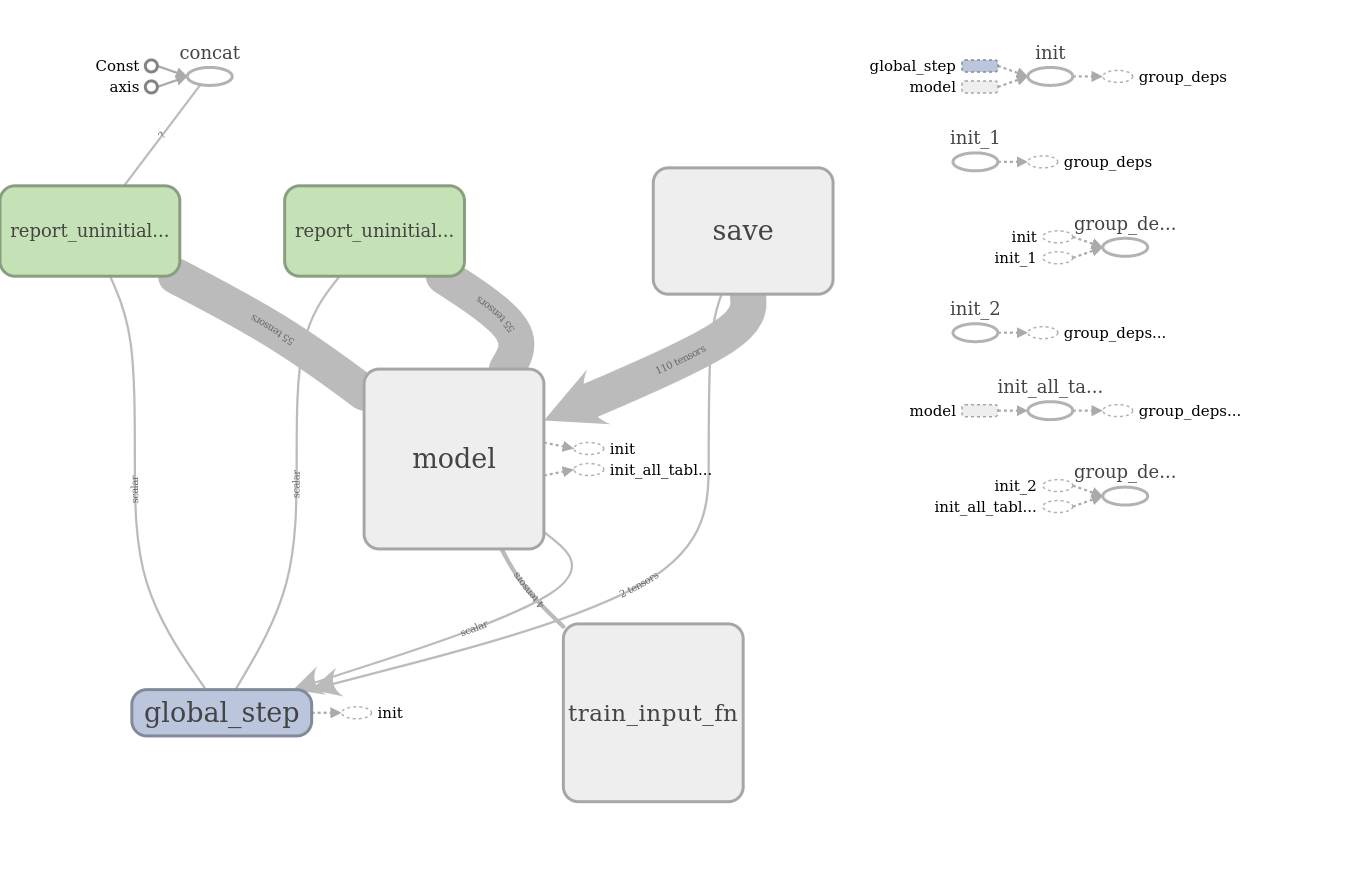
\includegraphics[scale=0.35]{example_graph.png}
	\caption{Computational Graph of tf-seq2seq model}
	\label{fg:exgraph}
\end{figure}

We can see that the neural network consists only of the model block, but we have assisting code that helps to make the model flexible and failure resistant.  In the Appendix of the paper, I include diagrams of the internals of the neural network, such as the layout of the Encoders and Decoders for some of the models.
\subsection{Small Model}
The small model was quite easy to train, and 

\begin{figure}[H]
	\centering
	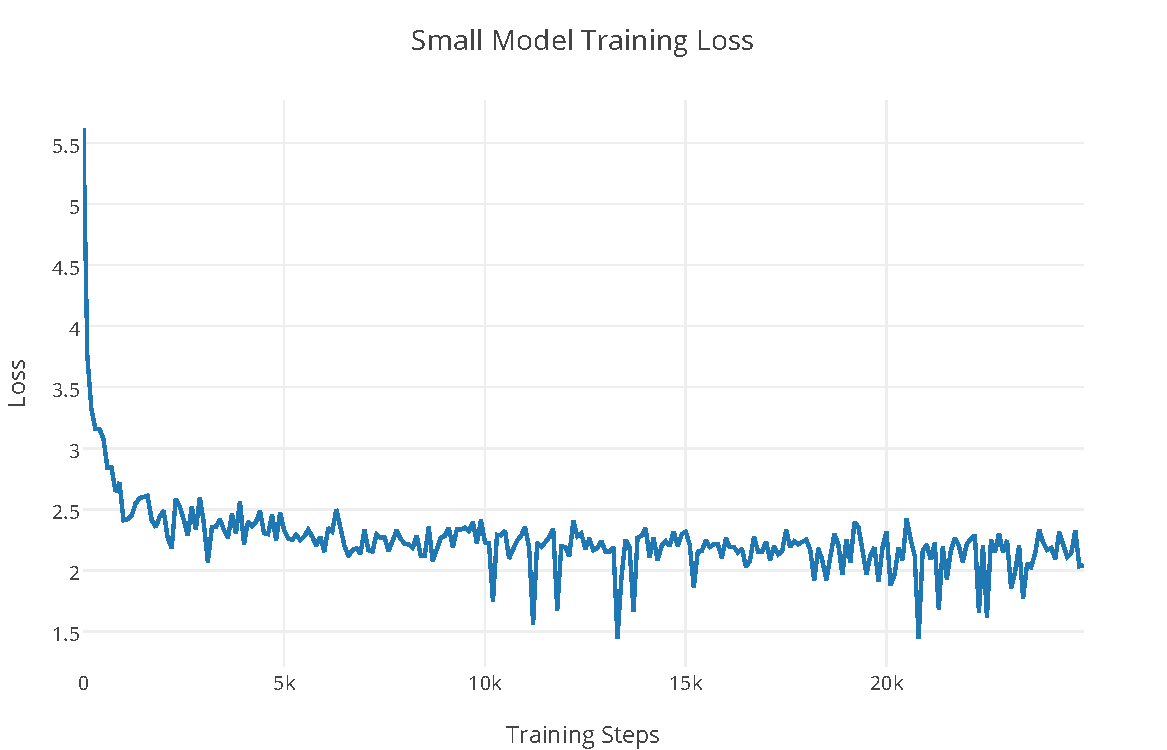
\includegraphics[scale=0.75]{Small_Loss.pdf}
	\caption{Training Loss Curve for Small Model}
	\label{fg:small_loss}
\end{figure}

\subsection{Medium Model}
The medium model was the hardest model to train, for reasons that will be explained in the Computation Time section.  Unfortunately, due to this, I was only able to train the medium model for  time steps.  While this initially sounds bad, the medium model has some of the fastest convergence behavior, converging to a loss in the low 2's.  This can be seen in the graph below

\subsection{Large Model}
The large model was surprisingly easy to train, but time consuming.  This model took approximately 16 hours to train to 2400 time steps.  As it was the largest of the three models, I ran it on the 16 GPU machine to give it the most GPU memory and processing power.  
\begin{figure}[H]
	\centering
	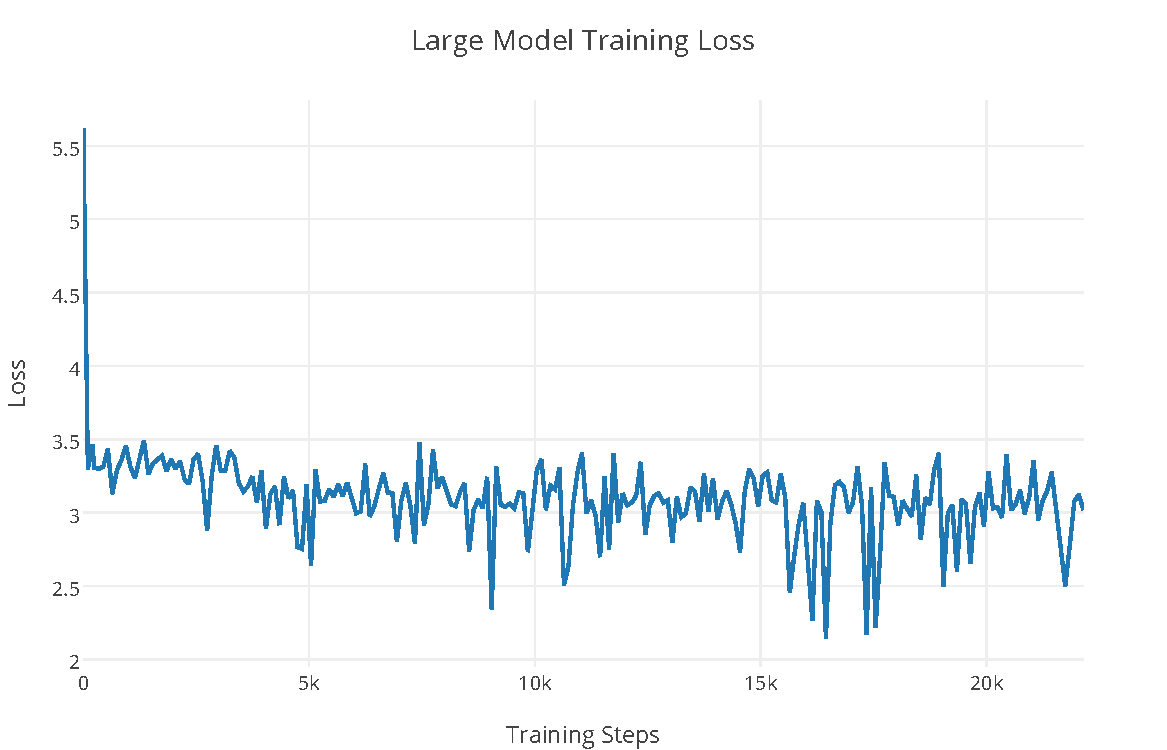
\includegraphics[scale=0.75]{Large_Loss.pdf}
	\caption{Training Loss Curve for Large Model}
	\label{fg:large_loss}
\end{figure}

\par
When examining the embedding average weights, I noticed that they trained particularly quickly in comparison to the rest of the model.  This is displayed in Figure \ref{fg:embed_avg} below.

\begin{figure}[H]
	\centering
	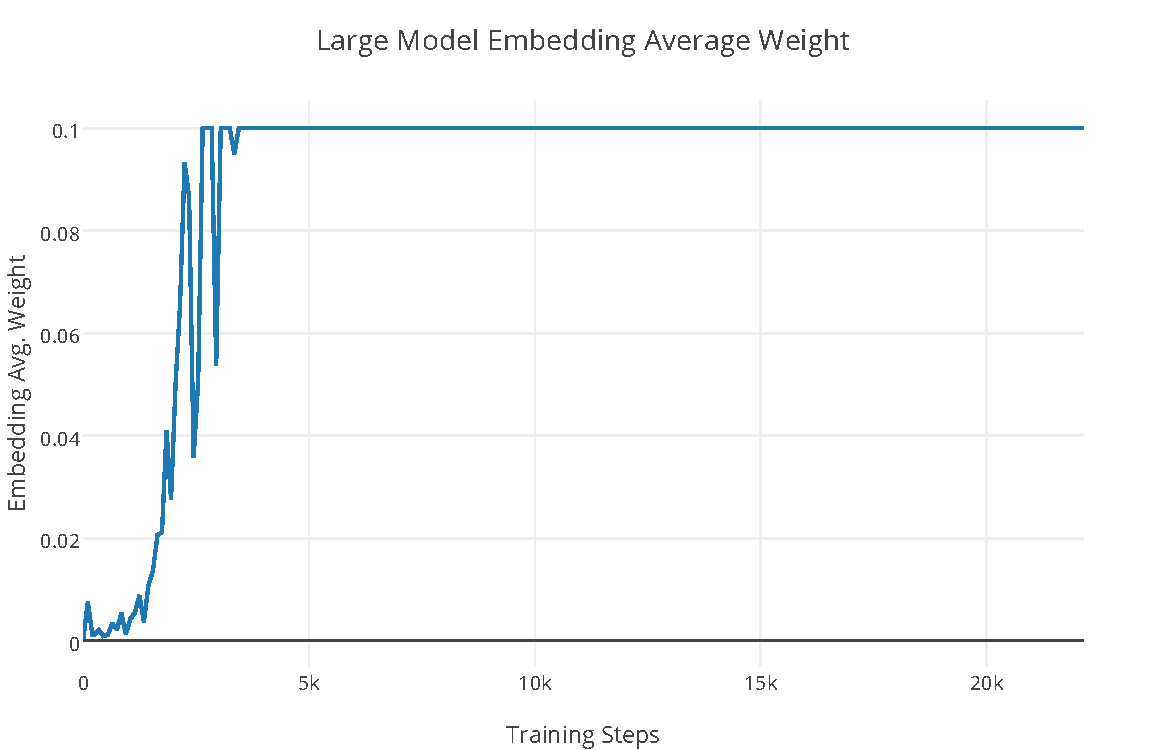
\includegraphics[scale=0.75]{Embedding_Avg_Weight.pdf}
	\caption{Embedding Avg Weight Training Curve}
	\label{fg:embed_avg}
\end{figure}

\subsection{Computation Time}
As mentioned earlier, to complete the training and inference of the networks, I had to run them on multiple machines, each with their own unique set of hardware specifications.  Therefore, any of the following time results must be viewed with this fact in mind.  However, provided below in the table are the number of training steps executed per second and how many GPU's available for training the model.

\begin{table}[H]
	\centering
	\caption{Computation Time for the three models}
	\label{tb:comp_time}
	\begin{tabular}{|l|l|l|l|l|}
		\hline
		\textbf{Model}  & \textbf{Service} & \textbf{\# GPUs} & \textbf{Avg. Steps / Sec} & \textbf{Steps / (GPU * Sec)} \\ \hline
		Small  & AWS     & 16      & 3.3              & 0.20625             \\ \hline
		Medium & Google  & 8       & 0.08             & 0.01                \\ \hline
		Large  & AWS     & 16      & 0.32             & 0.02                \\ \hline
	\end{tabular}
\end{table}

As we can see, the small model was able to train the fastest, training approximately 10 times faster than the large model on the same configuration and 20 times faster than the medium model.  This is expected as the Backpropagation through Time algorithm must only backpropagate the errors one layer back for each network.  Overall, I found that the small and large models trained in a reasonable amount of time, given the configuration of the server they were running on.  The medium model


\par
As a small note, I found the models trained on Google Compute Engine to be significantly slower for some unknown reason.  It seemed as if the Google instances had more lag in comparison to the Amazon Web Services instances.  I was unable to debug the problem, and as such the amount of time that the medium model could train for was reduced.  This is highly unexpected, since the tf-seq2seq code advertised a training time of 2-3 days for the large model, on 8 Nvidia K80 GPUs \cite{britz:2017}.  Given that they considered 5,000,000 training steps fully trained, and that the medium model is half the size of the large model, I find these training time claims to be highly inflated.  While the actual training times are still reasonable compared to other state of the art neural networks, I believe that the Google team should reexamine the runtime of the code in order to provide a much more reasonable estimate, or qualify their runtime with further data.

\subsection{Summary}
Although I did not train these models to the 5,000,000 training steps as done in the tf-seq2seq tutorial, I believe that the amount of training done was sufficient to extrapolate data from the models.  However, due to the flexibility of the tf-seq2seq software, the models can be trained further for any number of training steps, given the running files.  All code, datasets, and TensorFlow model files can be found in the github repository located at \url{https://github.com/PrincetonUniversity/ProtNet}.  By the time this paper is finished, it will be available to the public.  The final Q8 accuracies are displayed in Table \ref{tb:q8_accuracy} below.

\begin{table}[H]
	\centering
	\caption{Q8 Accuracy of the Models}
	\label{tb:q8_accuracy}
	\begin{tabular}{|l|l|}
		\hline
		\textbf{Model}  & \textbf{Q8 Accuracy} \\ \hline
		Small  &             \\ \hline
		Medium &             \\ \hline
		Large  &             \\ \hline
	\end{tabular}
\end{table}


\section{Conclusion}
Overall, I am quite satisfied with the results of this study.  From the accuracies achieved, we can clearly see that these models are capable of predicting secondary structure.  It would be worth studying these models further by tuning the hyperparameters better, finding ways to expand the dataset by using a better culling algorithm, or 

\par
For future work, I would like to investigate the incorporation of multiple alignment data in the input to the network.  Integrating multiple alignment data has been shown to be critical in improving the accuracy of secondary structure prediction.  It was originally suggested that I use this as my main architecture for this study; however, I wanted to focus on the ability for this type of network architecture to inference using only the input sequence.  One of the main difficulties is that it would require protein BLAST (BLASTP) to be packaged offline, as the network would prediction code would need to call BLASTP for every new protein sequence.  However, once this is done, one would have to change the network architecture to accept this extra alignment information.  I propose the following modifications to allow for this.  First, instead of using the embedding vectors on three-mers in the amino acid sequence, we use the embedding vectors to represent a single column of a protein alignment.  Consequently, this would mean that the number of embedding vectors to represent the entire sequence would be equal to the length of the amino acid sequence.  This would give the extra benefit of allowing the network to perform conformation prediction for individual amino acids instead of individual tri-mers.  One of the pitfalls, however, is that it will accept only a constant number of alignment proteins for a given input protein.  Furthermore, total vocabulary size of the embedding would increase significantly, as it must now include alignment symbols in each embedding "word".

\par
A convolutional model would be worth trying, as it strays from the standard LSTM based Encoder architecture..  Convolution is a complex mathematical operation that involves two functions.  In the case of neural networks, we treat the input as one of the functions.  The other input, called the kernel, is learned during training.  The benefit to using convolution in a neural network is that compared to more traditional neural networks, the number of learned parameters per layer, making the network more memory efficient and easier to train.  Convolutional based Encoder networks were first introduced in 2016 as a way to bring the benefits to convolution to Encoder / Decoder networks \cite{gehring:2016}.  A simple starter model to test this concept would be one where the Encoder would have a total of six convolutional layers, each with a kernel size of three.  Moreover, the Decoder would consist consists of one LSTM layer.


\par
One of the key difficulties training machine learning algorithms on secondary structure data is the comparably small size of the dataset in comparison to other tasks.  A simple way to compare this is by looking at the raw file size of the dataset.  While the entire PDB secondary structure dataset can be fit in a single \SI{196.7}{\mega\byte} FASTA file, where as standard text corpora range from as small as \SI{580}{\mega\byte} to as large as \SI{2.3}{\giga\byte}.  Even compared to the small text corpus, the secondary structure dataset is $\frac{1}{3}$ the size.  This might hinder the neural network, as it has to generalize over a smaller dataset.  In most cases, the easiest way to solve this problem is to gather more data.  As mentioned earlier, this is not feasible, due to the complex process of experimentally discovering the conformation of a protein.  A possible method to overcome this is a recent technique called generative adversarial networks, or adversarial learning.  First introduced by Ian Goodfellow in 2014, this technique uses two neural networks playing against each other in a zero-sum game \cite{goodfellow:2014}.  One network focuses on classification while the other tries to generate new datapoints.  Through this competition, both networks are able to learn the data not only through the provided training dataset, but through new data created by the generative network, given to the discriminative neural network.  The new data provided by the generative network is designed to maximize the probability that the discriminative network will mis-categorize the data.  This competition causes the generative network to provide harder and harder data to the discriminative network, which helps to increase the training accuracy of the discriminative network.  What makes this technique so enticing to the problem of secondary structure prediction is the generative capabilities of the network.  Because the network is able to generate example datapoints, we are able to train the network on a much larger, practical dataset.  One of the difficulties in this approach is the fact that adversarial networks built so far have been found to perform poorly on text-based problems.  Therefore, this would be a study to be performed once the network architecture improves.

% Bibliography
\pagebreak
\bstctlcite{bstctl:etal, bstctl:nodash, bstctl:simpurl}
\bibliographystyle{IEEEtranS}
\bibliography{references}
\pagebreak

\section{Appendix}
\begin{singlespace}
\begin{listing}
\inputminted[]{YAML}{../config/small_config.yaml}
\caption{YAML configuration file for small network model}
\end{listing}
\pagebreak

\begin{listing}
\inputminted[]{YAML}{../config/medium_config.yaml}
\caption{YAML configuration file for medium network model}
\end{listing}
\pagebreak

\begin{listing}
\inputminted[]{YAML}{../config/large_config.yaml}
\caption{YAML configuration file for large network model}
\end{listing}
\pagebreak

\begin{listing}
	\inputminted[]{YAML}{../config/conv_config.yaml}
	\caption{YAML configuration file for convolutional network model}
\end{listing}
\pagebreak
\end{singlespace}

\pagebreak
\begin{figure}[H]
	\centering
	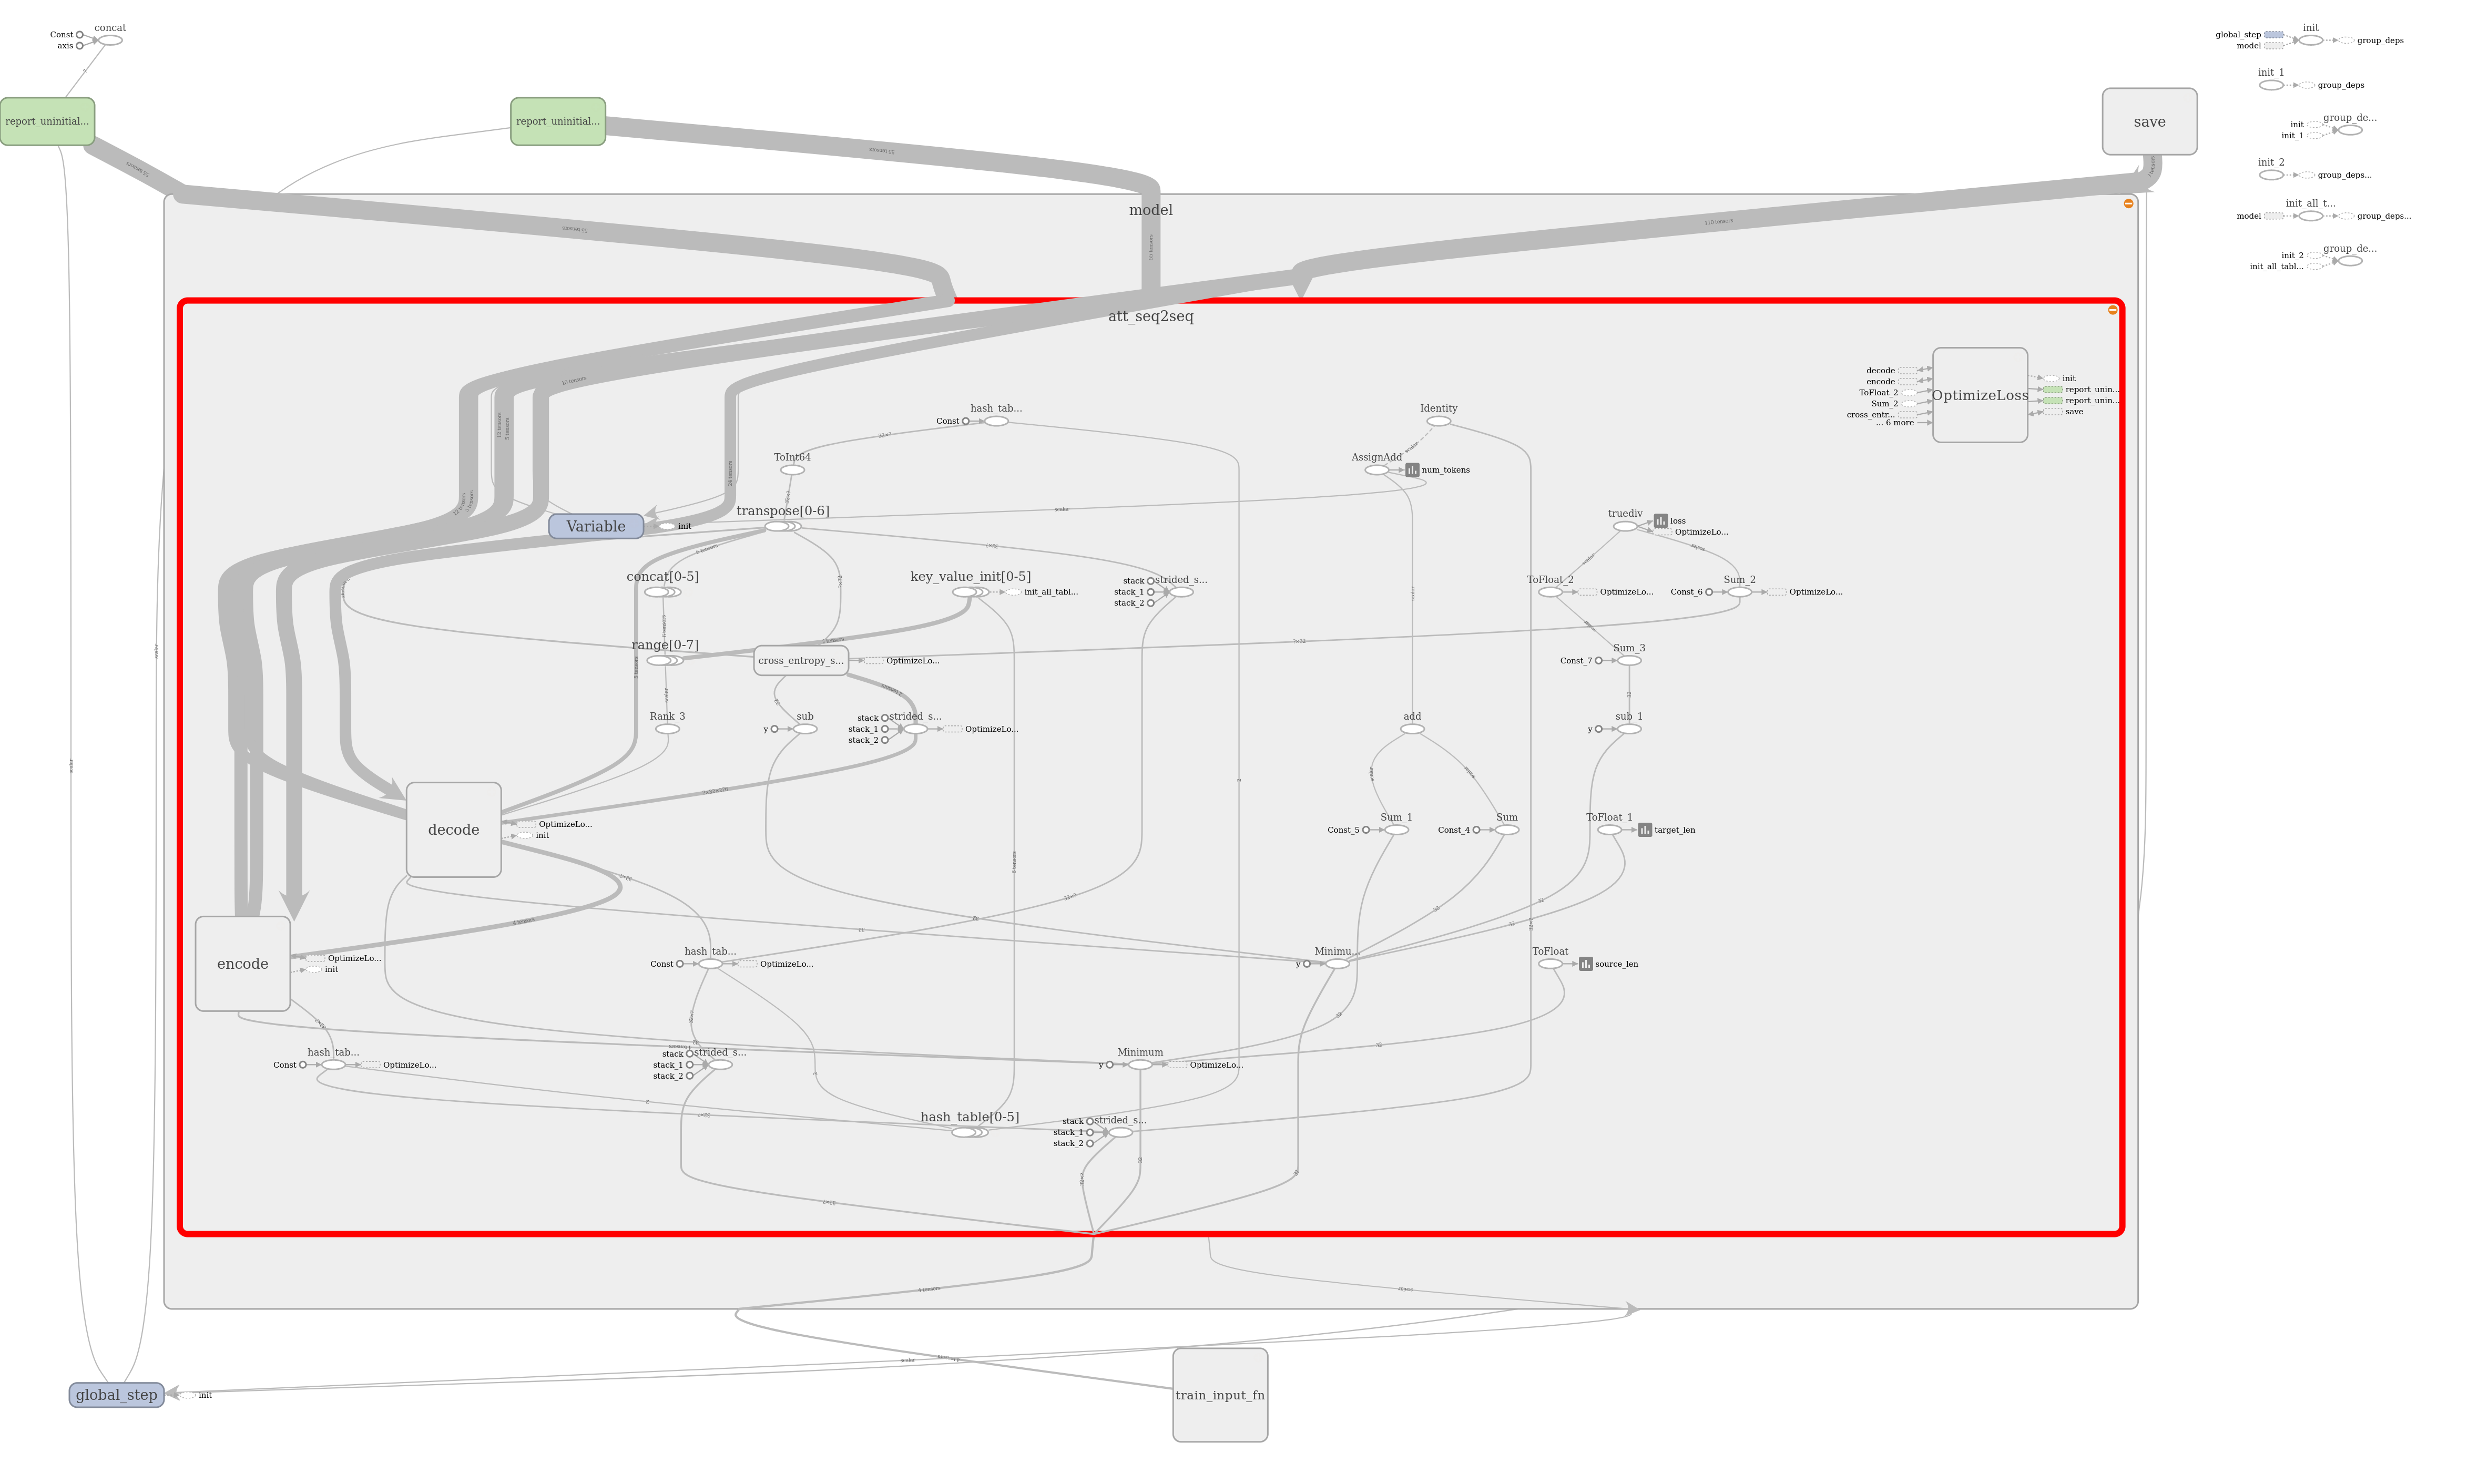
\includegraphics[scale=0.13, angle=90]{small_model_full_graph.png}
	\caption{Computational Graph of Large Model}
	\label{fg:small_model_graph}
\end{figure}
\pagebreak

\begin{figure}[H]
	\centering
	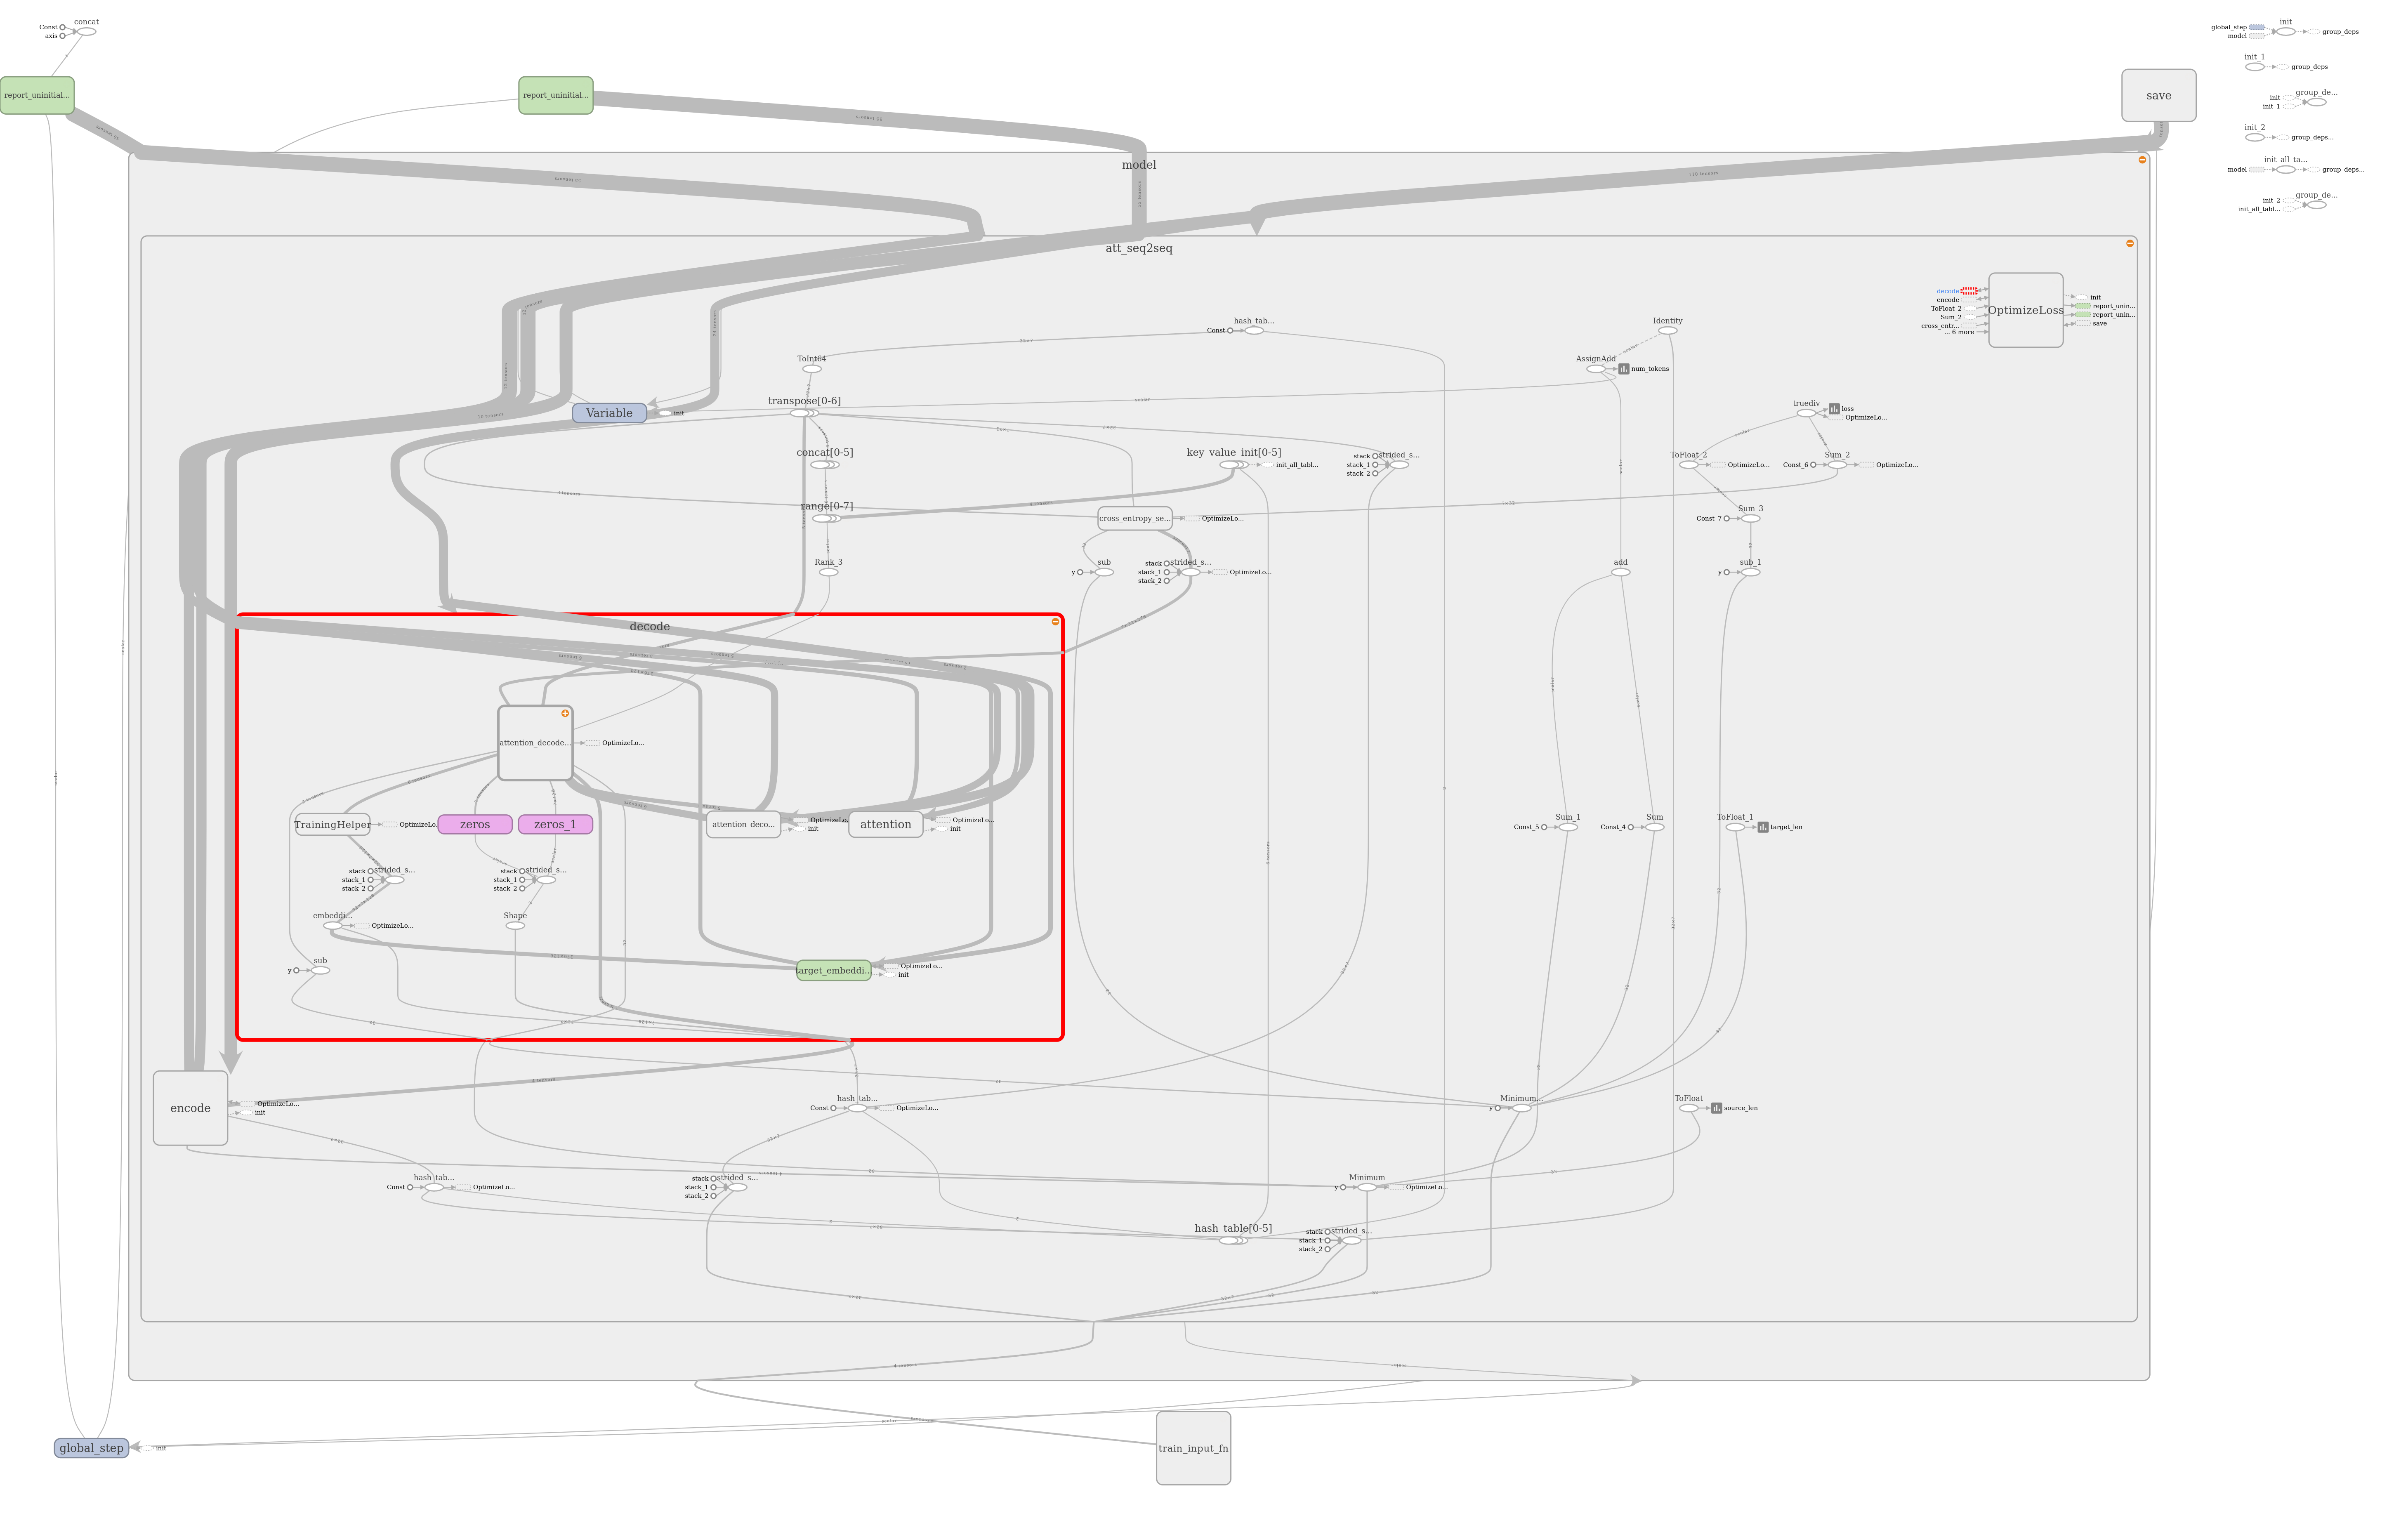
\includegraphics[scale=0.103, angle=90]{small_graph_decoder.png}
	\caption{Computational Graph of Large Model Decoder}
	\label{fg:large_model_decoder_graph}
\end{figure}

\end{document}

